\documentclass[a4paper,12pt,english]{article}
 
\usepackage[utf8]{inputenc}
\usepackage[T1]{fontenc}
\usepackage{babel}

\usepackage{hyperref}
\def\UrlBreaks{\do\/\do-}
\usepackage{graphicx}
\usepackage{wrapfig}
\usepackage[table,xcdraw]{xcolor}

\usepackage{cite}
\usepackage[inline]{enumitem} % inline lists
\usepackage{caption}
\usepackage{subcaption}
\usepackage{float}
\usepackage{fancyvrb}
\newcommand{\infra}{\emph{infra}}
\newcommand{\TODO}{\fbox{\textcolor{red}{TODO}}}

\begin{document}

\begin{titlepage}
	\centering
	\fbox{\begin{minipage}{\textwidth}
	\centering
	\vspace{0.3cm}
    {\scshape\LARGE\bfseries Project Report\par}
	\vspace{0.2cm}
	{\Large\bfseries Automated Essay Scoring \par}
	\vspace{0.3cm}
    \end{minipage}}
	
	\vfill
	
\includegraphics[width=0.5\textwidth]{fig/psl.jpg}\par\vspace{0cm}
	{\scshape\Large IASD Master \par}
	\vfill
	{\Large Pierre-François \textsc{Massiani}\par}
	{\Large Guillaume \textsc{Le Moing}\par}
	\vfill
	work completed during the\par
	Natural Language Processing class
	\vfill
    {\large April 25\textsuperscript{th}  , 2020\par}
\end{titlepage}
\tableofcontents
\newpage

\section{Introduction}

This is the final project for the « Natural Language Processing » class of Master IASD (Artificial Intelligence, Systems, Data), a joint PSL University Master program hosted by Paris-Dauphine, École normale supérieure, and MINES ParisTech.

In this project we propose and compare different neural network architectures as well as learning strategies for the automated essay scoring task.
We test our algorithms using the data from the ASAP competition on Kaggle~\cite{kaggle} sponsored by The Hewlett Foundation.

Our project was implemented in Python. The code is available on a Github repository at this address:
\begin{center}
	\url{https://github.com/16lemoing/automated-essay-scoring/} 
\end{center}
Instructions are included in the repository to run the code on your machine.

\subsection{The automated essay scoring task}
The task we are trying to solve here is called \emph{automated essay scoring} (AES). It consists in automatically assigning a grade to an essay written on a given topic. This is of particular interest in an educational setting, where incentives for developing unified and objective grading methods can be easily understood. Such a method could be used for instance to grade large scale exams where teachers need to evaluate hundreds of essays in a short amount of time, leading to exhaustion, unwanted bias introduced by how focused the teacher is when reading, and discrepancies in the grades caused by the teachers' own evaluation criteria. Using an automated grading system can then help to standardize this process. For example, writing tasks were suppressed from French PACES\footnote{"Première année commune des études de santé", the first year of health studies in France.} competitive exam this year because teachers will not have enough time to grade them because of the coronavirus outbreak\cite{paces}. An automated grading system could help to solve such problems. Other factors also account for the growing interest in this task, such as cost reduction.\par
In spite of these incentives pushing for the development of automatic essay scoring algorithms, the attempts at using them received quite a backlash. The arguments against these algorithms were that they did not understand the meaning of the essays they were grading and were relying only on "surface features of responses". To prove their point, protestors created essays exploiting the biases discovered in the algorithm to create nonsensical high-graded essays. According to MIT Director of Writing Les Perelman, "the substance of an argument doesn’t matter [for such algorithms], as long as it looks to the computer as if it’s nicely argued"\cite{nyt2012}. Indeed, high grades were given to essays containing assertions that were simply not true, such as stating that the War of 1812 started in 1945.
\paragraph{The Hewlett Foundation challenge} In 2012, \emph{The Hewlett Foundation}\footnote{The Hewlett Foundation is a private foundation that grants awards in a variety of liberal and progressive causes such as education, climate, health, journalism...} sponsored a competition on Kaggle\cite{kaggle} intended at demonstrating how AES algorithms - and more specifically neural networks - could be as reliable as humans in rating thousands of essays. Although this competition was very successful\cite{nguyen2018neural,song2013automated,turanga,chanakya}, it is still controversial whether the initial claim is backed up by the competition's results. In this project, we propose an algorithm for the Hewlett Foundation's challenge.

\subsection{Related work}
The interest for the AES task sparks around 1970 with the works of Ellis Batten Page\cite{page1966imminence}, but it quickly faces the limitations imposed by the computational power available at the time. This practical limitation is lifted in the 1990s, and 1999 sees the first commercial automatic essay grader\cite{attali2004automated}. After that, the field grows rapidly and different approaches are tested with the state-of-the-art statistical inference techniques known at the time\cite{rudner2002automated}.\par
Today, the AES task is typically tackled using modern and state-of-the-art natural language processing (NLP) tools. Indeed, AES is a subtask of the more general text classification problem, which is a vibrant field in the NLP community. As such, classical NLP techniques can be used to achieve great results such as dense neural networks\cite{murray2012automatic}, convolutional networks\cite{kim2014convolutional}, or recurrent networks\cite{taghipour2016neural}.

\section{A Neural Network based approach}

We choose to rely on neural networks for this task.
We describe in this section the whole pipeline from raw essays to the prediction of the scores.
For each part, we present different options that are included in this project.

\subsection{Words embedding}
Essays have to be turned into vectors of numbers before being fed to a neural network.
One popular strategy is to assign a vector to every single word in the text.
The required dimension for the vectors depends on the richness of the vocabulary (both in quantity and lexical diversity).
\subsubsection{Random}
This is the most basic embedding.
We assign to each word of the vocabulary a vector of random samples from a normal (Gaussian) distribution.
\subsubsection{Word2Vec}
We propose to train a Word2Vec model~\cite{mikolov2013efficient} on the sentences extracted from the training essays.
This model learns meaningful embeddings by trying to guess a word from its context (a few words before and after in the sentence).
To do this each word of the context is turned into a vector from which the prediction is made.
Those vectors are what we use as embeddings once the model is trained.
Each set of essays deals with a different topic.
We hope to capture topic-related knowledge from the corpora by learning the embedding directly from the set of training essays.
\subsubsection{GloVe}
We also propose a different strategy for getting word embeddings using GloVe~\cite{pennington2014glove}.
The particularity of GloVe embedding is that there are linear substructures between words sharing semantic aspects.
For this embedding, we decide not to train the GloVe model from scratch but use a pre-trained model on large-scale corpora such as Wikipedia instead.

\subsection{Essay preprocessing}
We present here a few preprocessing methods that can help the learning process.
\subsubsection{Spelling errors correction}
Reading a few essays, we realised that there were lots of misspelled words in the essays.
This can impair the prediction performance because we cannot provide a meaningful embedding to misspelled words and we have a much larger vocabulary.
It would have come in handy to have a python wrapper for a correction tool such as LanguageTool which handles both syntaxic and grammatical errors.
Instead we used pyspellchecker package which gives a list of the most plausible correction candidates for each of the misspelled words (but do not consider the sentence as a whole).
\subsubsection{Stopwords removal}
There are some very common words, called stopwords that usually do not add much meaning to the sentence.
A common preprocessing step in natural language processing consists in removing these words that can pollute the learning process.
However, in our case it is unclear whether we should remove these words or not.
For example we need to take them into account when evaluating the gramatical correctness of a sentence.
That being said, it would be surprising that our model learns what is a grammaticaly correct sentence from such a small corpus.

\subsection{Essay processing}
We describe here how the essays are transformed so that they can be understood by a neural network.
\subsubsection{Word tokenization}
The first step is to transform essays into tokens (isolated words).
To do that we transform every special character into a space symbol and then split the essay at every occurence of the space symbol.
\subsubsection{Essay padded encoding}
Then we assign to each word its index in the vocabulary. This index will be used as a key when retrieving the word embedding.
To enable batch-learning we pad every essay so that it matches the length of the longest essay.

\subsection{Multitask model}
The dataset contains multiple essay tasks which are scored on different scales.
This makes it difficult to learn all tasks jointly.
However this can be addressed by normalizing the scores.
\subsubsection{Score normalization}
We rescale all the scores so that they fall into $[0,1]$, by applying this simple linear transformation:
\begin{equation}
s_{norm} = (s - s_{min}) / (s_{max} - s_{min})
\end{equation}
\subsubsection{Score recovering}
For the evaluation we need to recover the score in its original scale.
To do this we apply the inverse transformation and then round the obtained value to the nearest score value in the corresponding set.

\subsection{Extra-features computation}
\label{pos:extrafeats}
When predicting a score for an essay it is possible to include higher-level features to give some insights about characteristics that are hard to grasp for the neural network.
First, during the spelling correction, we can compute the number of misspelled words for each essay. Doing this, the model can be fed the corrected essays and have a better understanding of the meaning while still being able to judge on this aspect.
We also extract part of speech indicators from the essays (number of nouns, adjectives, verbs...), usage of ponctuation (number of question marks, exclamation marks, commas...), semantic diversity (number of semantic roots that were used to build the words in the essay), quotations (counting quotation marks, references to organizations, locations, people...).

\subsection{Models architecture}
We propose highly customizable neural networks to optimize there architecture based on the validation results.
\subsubsection{Dense}
\label{pos:densearchi}
First, we propose a four-layer dense neural network.
The first layer is the embedding layer.
We then take the mean of all the embedding vectors and feed it to a series of dense layers.
We use ReLu activation functions except for the output layer which has a Sigmoid activation when the scores are rescaled to $[0,1]$.
There is the possibility to add some dropouts between layers to prevent overfitting.
The dense model can be fed encoded essays, encoded essays + extra-features, extra-features alone.
This way we can evaluate the predictive power of each individual part.
\subsubsection{LSTM}
The dense neural network merges all word embeddings into a single vector.
It does not take into account the order in which the words appear in the essay.
We introduce an LSTM model so that we can work directly with sequenced data.
Our LSTM model is made of a custom number of layers and can include dropout.
We also add a few fully connected layers so that we can make use of the extra-features if they are provided.
\subsubsection{CNN}
Pursuing on our considerations on the strucutre of the text, we also propose a convolutional model. Convolutional architectures are very popular in image analysis tasks, because they can detect local patterns in the input data, and can adapt to different input sizes. Our architecture is inspired from the famous work of Kim et al.\cite{kim2014convolutional}. The embeddings are fed into three parallel 2D-convolution layers with kernels of different shapes. Our implementation chose kernels of size 3,4 and 5 along the time axis, and covering the whole embedding (see Figure~\ref{kim2014figure}). After that, we apply max pooling along the time axis for each channel, and feed the resulting nodes into a fully connected layer. This architecture has the advantage of being able to adapt to any essay length (thanks to the pooling), and should be able to detect syntactical richness thanks to the convolutional layers that shed light onto the local structure of the input.
\begin{figure}
	\centering
	% \hspace{-1.5cm}
	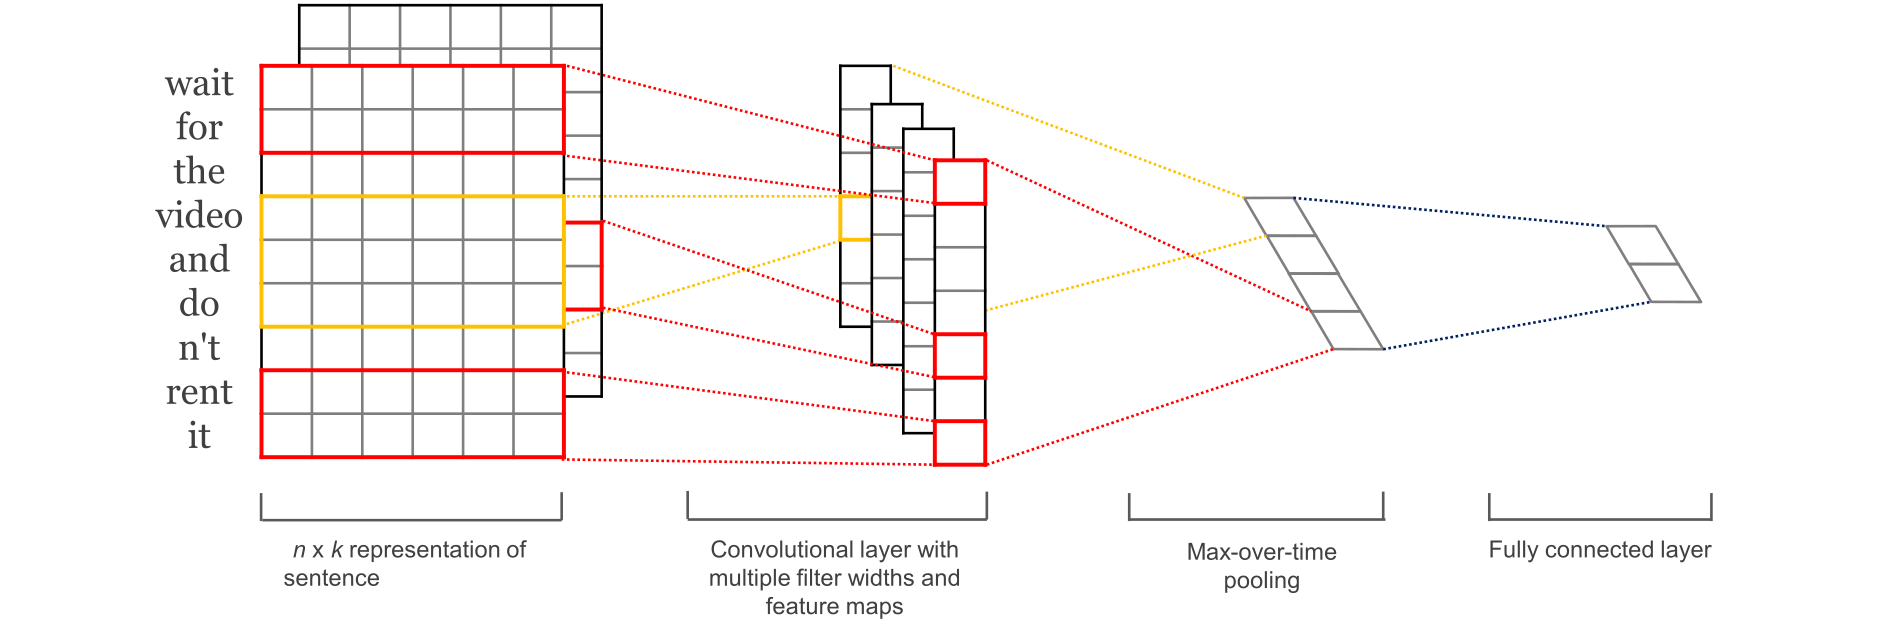
\includegraphics[width=\textwidth]{fig/kim2014fig.png}
	\caption{The architecture of the convolutional network\cite{kim2014convolutional}}
	\label{kim2014figure}
\end{figure}

\section{Experiments}
We conduct a thorough analysis to compare and discuss all the proposed learning strategies.

\subsection{Dataset}
The dataset we work on can be downloaded on the competition's website\cite{kaggle}, along with explanations on the essays and the (human) grading methods.
\paragraph{Essays description} There are eight essay sets, each generated from a single prompt: each set was created by collecting essays from students who worked on a particular topic. Hence, topics are \emph{coherent} among one set, and so is grading. The instructions across sets vary a lot : some essays are argumentative and should defend a point about something (e.g., "the effects on computers on people"), and others consist in text commentary. More details are given on each set in Table~\ref{setsdescription}. All essays were written by Grade 7 to Grade 10 students, and hand graded and double-scored. What's more, essays are graded on different criteria and, depending on the set, a detailed score is given as well as how to compute the global score from the detailed one.

\begin{table}
	\centering
	\begin{tabular}{llllll}
	\hline
	Essay set & Type & Set size & Average length & Range 1 & Range 2\\
	\hline
	1 & Argumentative & 1785 & 350 & 1-6 & 2-12\\
	2 & Argumentative & 1800 & 350 & 1-6 & 1-4\\
	3 & Source based  & 1720 & 150 & 0-3 & -\\
	4 & Source based  & 1772 & 150 & 0-3 & -\\
	5 & Source based  & 1805 & 150 & 0-4 & -\\
	6 & Source based  & 1800 & 150 & 0-4 & -\\
	7 & Argumentative & 1730 & 250 & 0-15 & 0-30\\
	8 & Argumentative & 918  & 650 & 0-30 & 0-60\\
	\hline
	\end{tabular}
	\caption{Some statistics about the essay sets. A source essay is provided for all "Source-based" essay. The scoring methods are quite complex and are described more thoroughly in Section~\ref{validation}. The scoring ranges provided are used for detailed scores or global ones.}
	\label{setsdescription}
\end{table}

\paragraph{Dataset} The dataset comes with the following fields:
\begin{itemize}
	\item \verb|essay_id| An essay identifier, unique for each essay
	\item \verb|essay_set| 1-8, an identifier for each set of essays
	\item \verb|essay| The text of the essay, encoded in ASCII
	\item Fields describing the detailed and global scores: 
	\begin{itemize}
		\item \verb|rater1_domain1|, \verb|rater2_domain1|, \verb|rater3_domain1| Domain 1 score for each rater
		\item \verb|domain1_score| Resolved Domain 1 score
		\item \verb|rater1_domain2|, \verb|rater2_domain2| Domain 2 score for each rater~\footnote{Only for Set 2.}
		\item \verb|domain2_score| Resolved Domain 2\footnote{Only for Set 2.}
		\item \verb|rater1_trait1_score| - \verb|rater3_trait6_score| Trait scores\footnote{Only for Sets 7 and 8.}
	\end{itemize}
\end{itemize}
The scoring fields are missing in the validation and test sets. However, we absolutely need them in order to first train, and then evaluate our models. Hence, we only work on the competition's training set and we divide it into our own training, validation and test sets. What's more, we do not follow the formatting of the output as it is described on the competition's website, since it is not required for this project. 
\subparagraph{A note on anonymization} The essays may mention names, dates, locations, organizations, etc. Such mentions were replaced before the publication of the dataset with easily identifiable keywords to anonymize the essay: we will keep that in mind when designing our algorithm.

\paragraph{Additional features} In the raw dataset, the only features we can use for prediction are the set number and the raw ASCII text. As described in Section~\ref{pos:extrafeats}, we start by enriching the dataset with extra features we compute from the text itself. The enriched dataset is generally denoted with the suffix \verb|_x| in our files, and is the one we use for prediction.
\subsection{Validation metrics}
\label{validation}
\TODO{présentation de la loss MSE}
\TODO{présentation du quadratic weighted kappa}
%dire que c'est la métrique que tout le monde utilise (dans le challenge aussi)
%on prend la somme pondérée du Quadratic Weighted Kappa pour chaque type d'essai (1 à 8) pour avoir la valeur finale
%on peut s'inspirer de
%https://cs224d.stanford.edu/reports/huyenn.pdf
%par ex

\subsection{Experimental protocol}
To compare all the configurations we use 5-fold cross-validation on the training data (for each fold the training data is split into subtraining and subvalidation sets)
The best epoch is found by looking at the lowest loss value on the subvalidation set.
We save the average validation metrics across all folds corresponding to the best epoch for each fold.
When all configurations have been cross-validated we test the best configuration on the test data (which remained unseen up to this point).

\subsection{Results}
All the results for the experiments are saved as things progress in an excel spreadsheet. The raw file containing all these results can be found at \verb+doc/raw_results.xlsx+ in the Github repository coming alongside with this report.

\subsubsection{Model selection}
In this first part, we describe the process we followed to find our best-performing model.

\paragraph{Pipeline optimization} First we show incremental results of pipeline features optimization compared to a baseline method. The baseline method corresponds to the set of default arguments (Word2Vec embedding of dim 50, shallow fully-connected model without dropout, no extra features, no special data preprocessing, learning from all essay sets at once). We found that the baseline method was rather unstable (sometimes giving decent results, sometimes not converging at all). Normalizing score so that they fit in $[0, 1]$ enabled a great improvement of the quadratic weighted kappa metric compared to the baseline method. Spelling correction led to maginally better scores. Extra-features insertion led to more instabilities but adding this together with feature scaling solved this issue and further improved the results. Changing the embedding dimension from 50 to 300 and removing stopwords helped improving the validation metrics even more.

\begin{center}
\vspace*{-1.5cm}
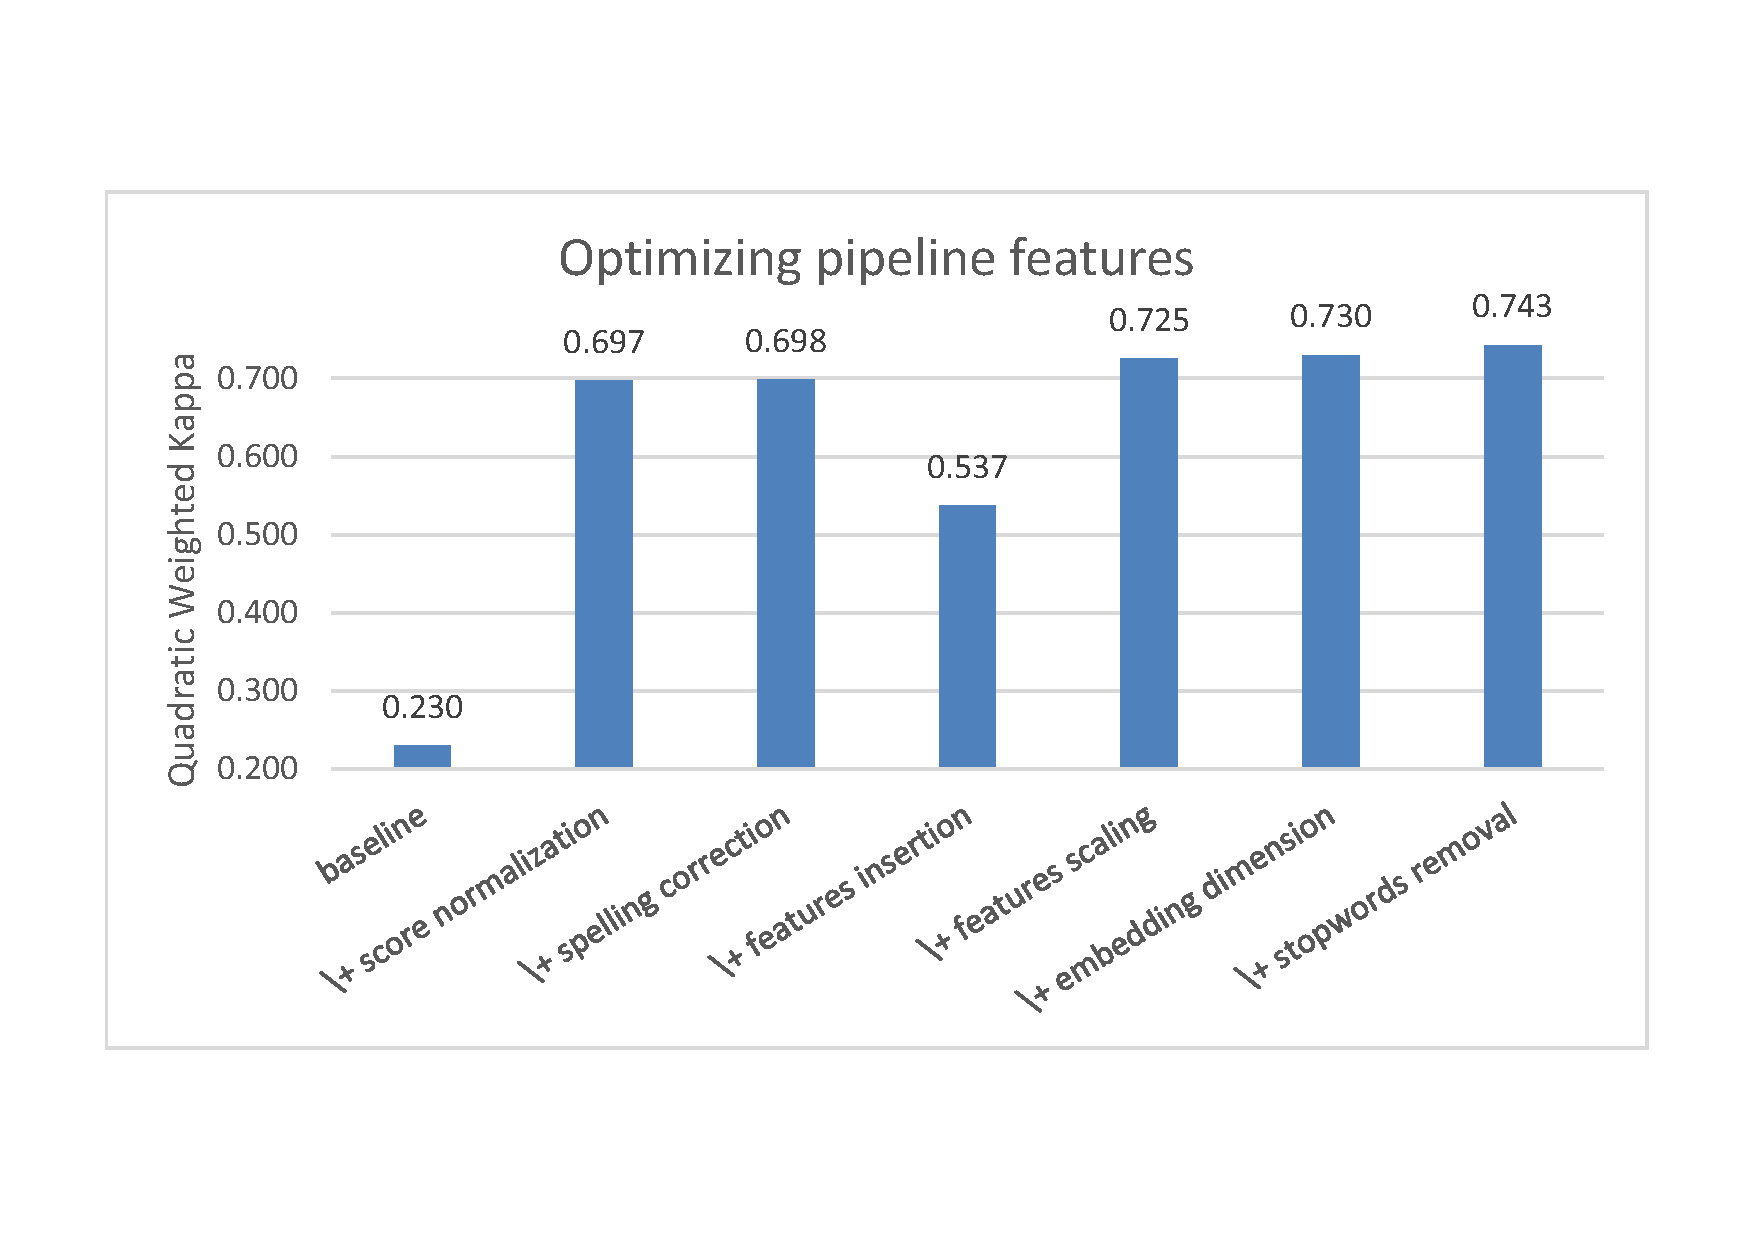
\includegraphics[width=0.85\textwidth]{fig/opt_pip_feat.pdf}
\vspace*{-1.5cm}
\end{center}

\paragraph{Hyperparameters tuning} Then we focused on tuning the key learning hyperparameters. For the choice of the learning rate, two values ($0.001$ and $0.01$) led to similar results. We selected $0.01$ because it was slightly better. For the batch size, results indicated that we should select either a small batch size or a very large one. As it speeds up the learning process we decided to go with a rather large batch size ($256$).

\begin{center}
\vspace*{-1.5cm}
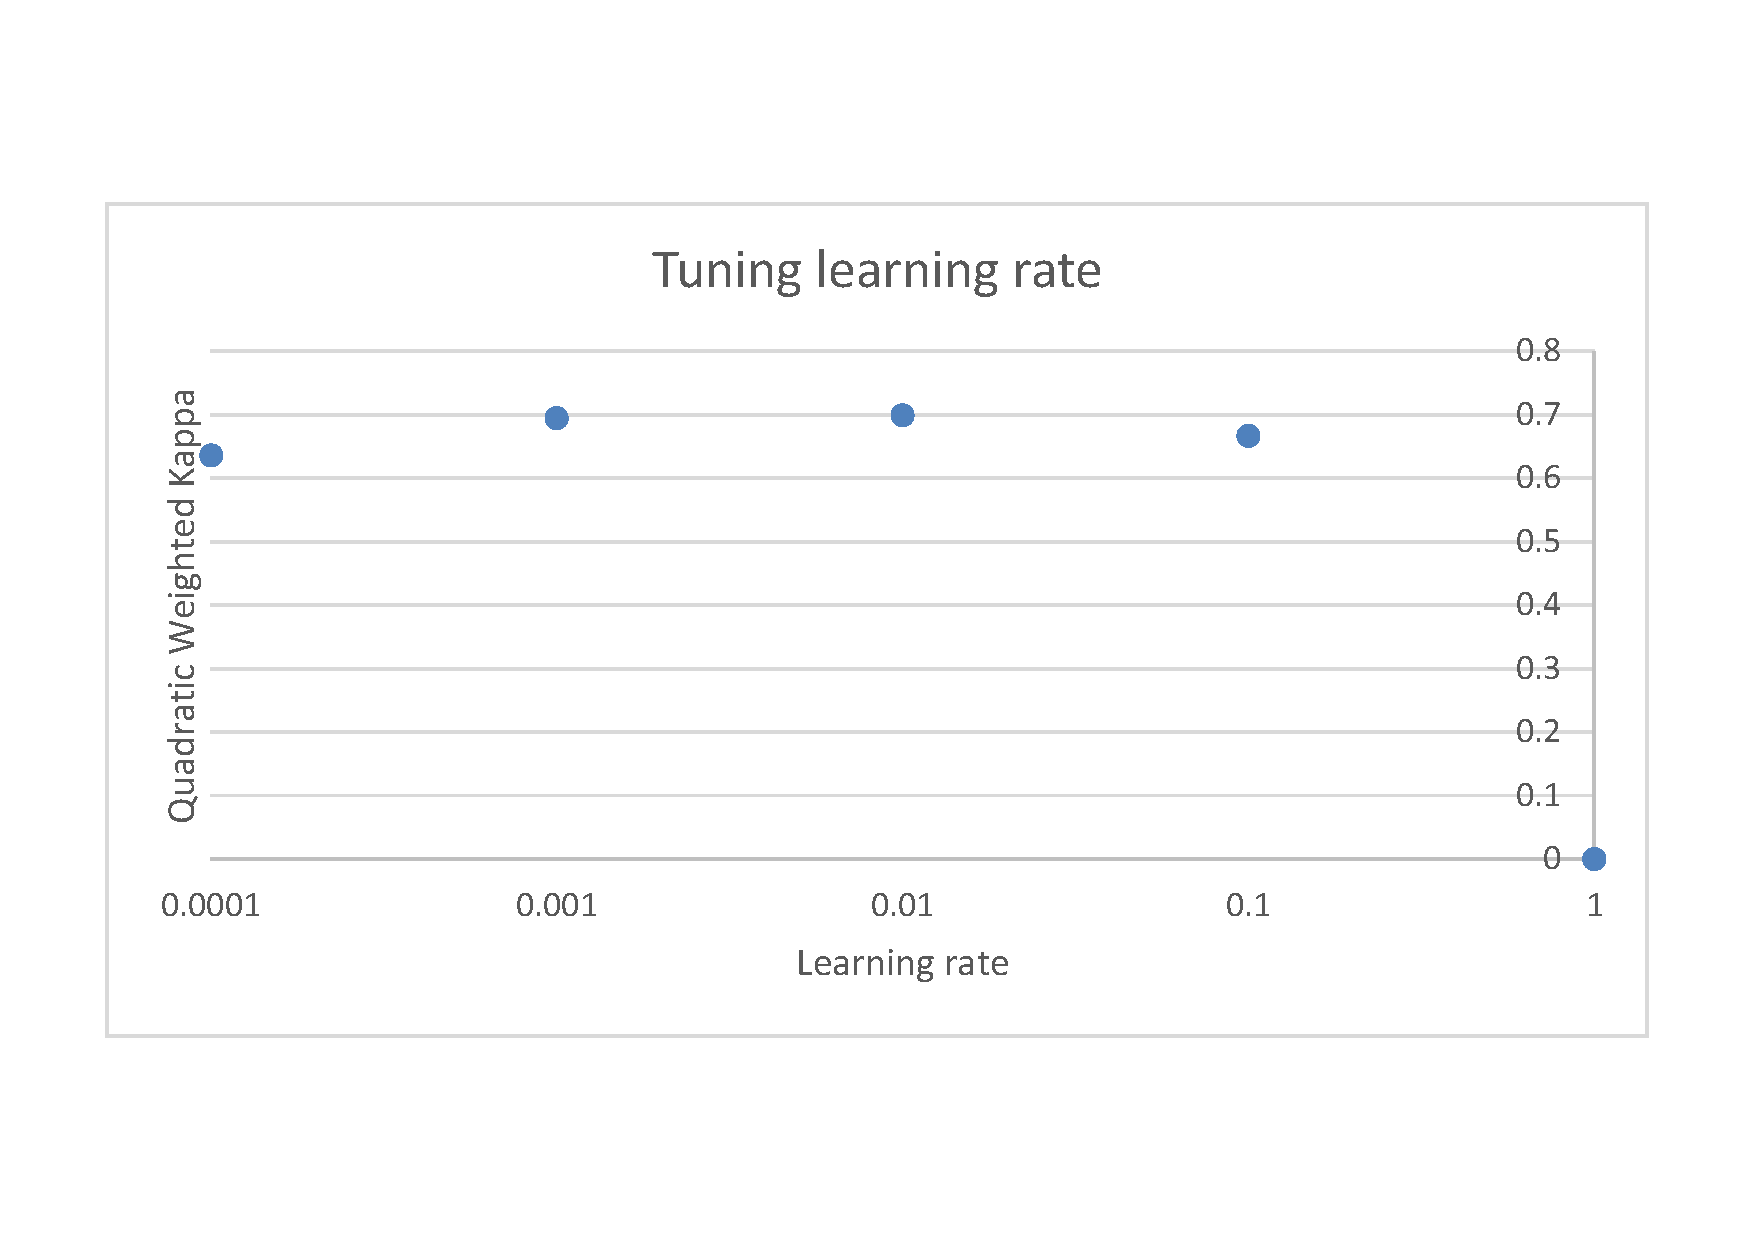
\includegraphics[width=0.85\textwidth]{fig/tune_lr.pdf}
\vspace*{-1.5cm}
\end{center}

\begin{center}
\vspace*{-1.5cm}
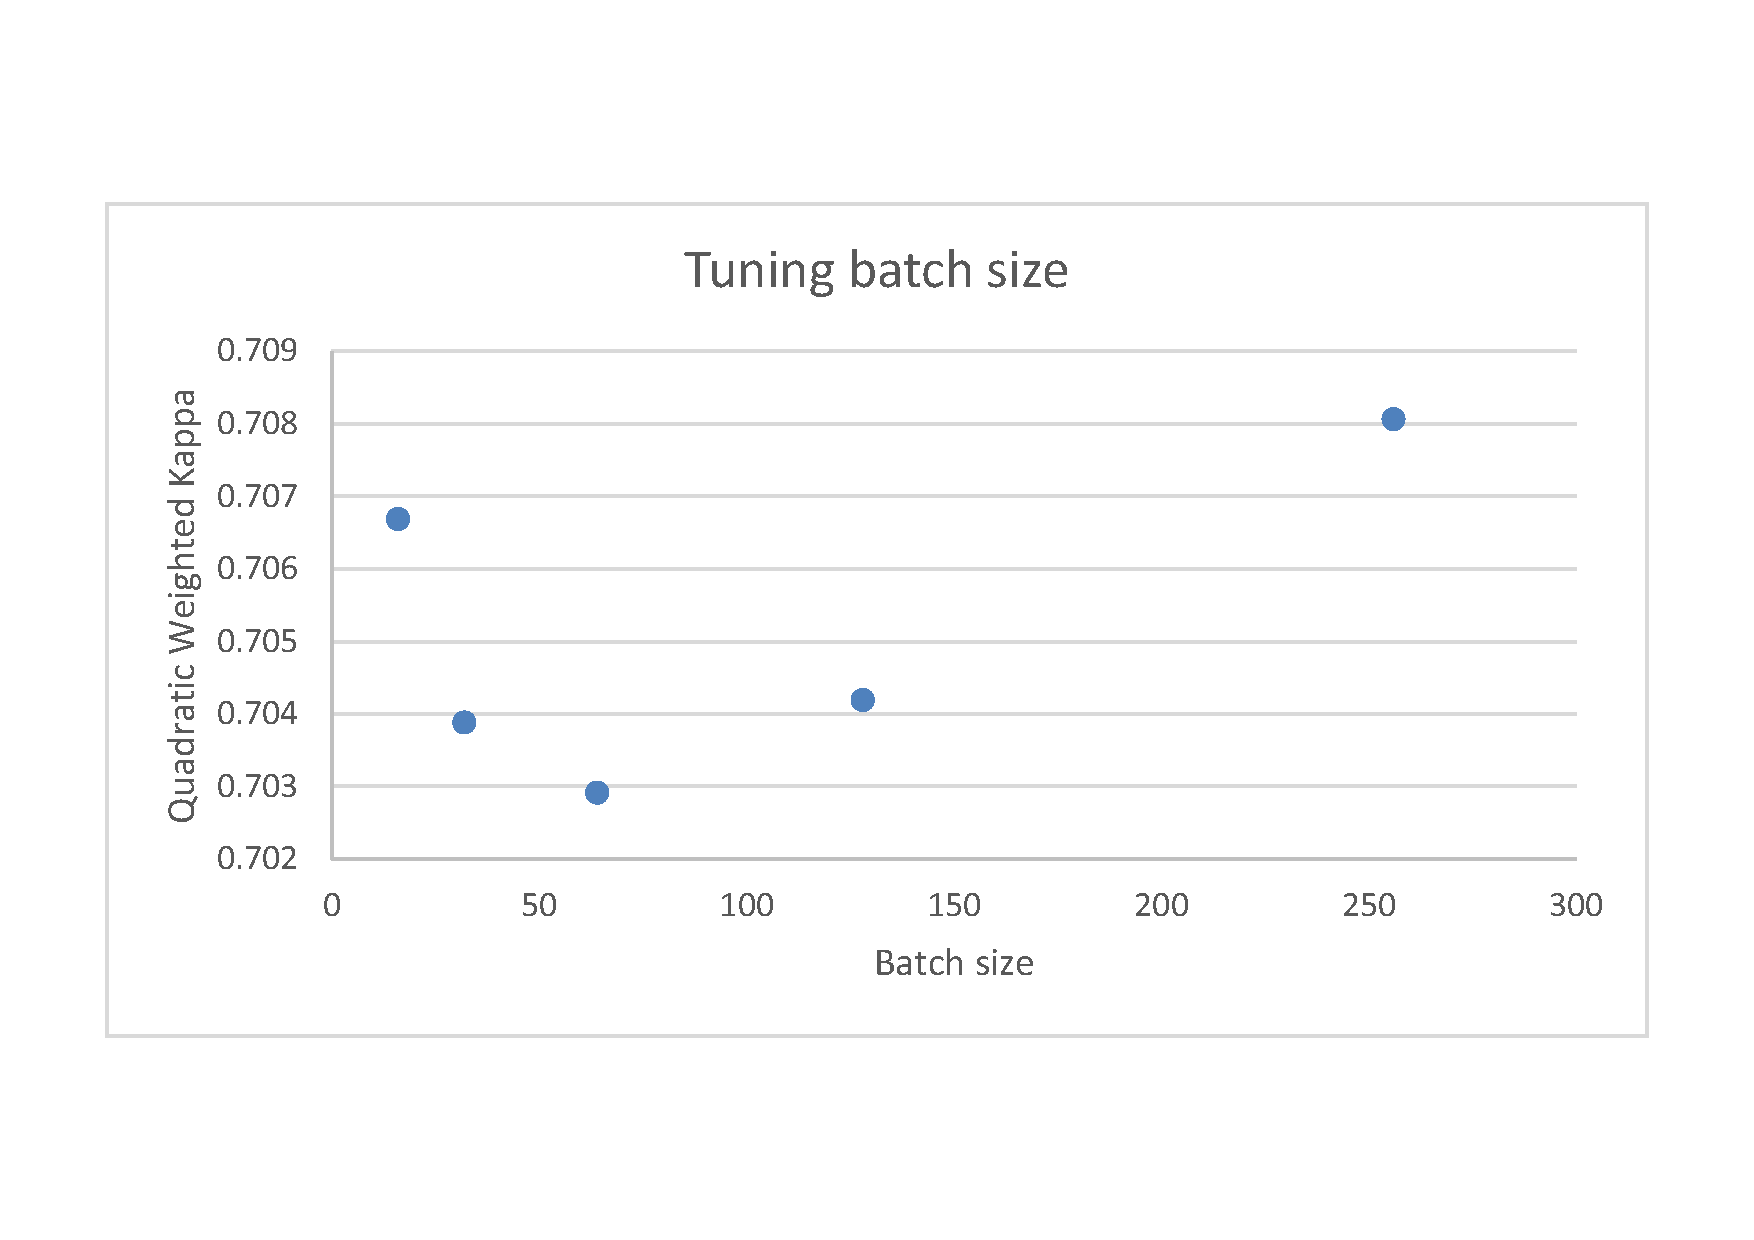
\includegraphics[width=0.85\textwidth]{fig/tune_bs.pdf}
\vspace*{-1.5cm}
\end{center}

\paragraph{Dense model optimization} We tried various architecture for the fully connected model. We show the results for different dropout values and number of parameters. The results shown correspond to learning from embedded essays as well as extra-features. We also tried learning solely from extra-features a reached a quadratic weighted kappa value of $0.678$ which is far from the best results we can get when combining embedded essays and extra-features. The best configuration for the dense model is obtained with hidden layers of size $300$ and $128$ and dropout of $0.2$.

\begin{center}
\vspace*{-1.5cm}
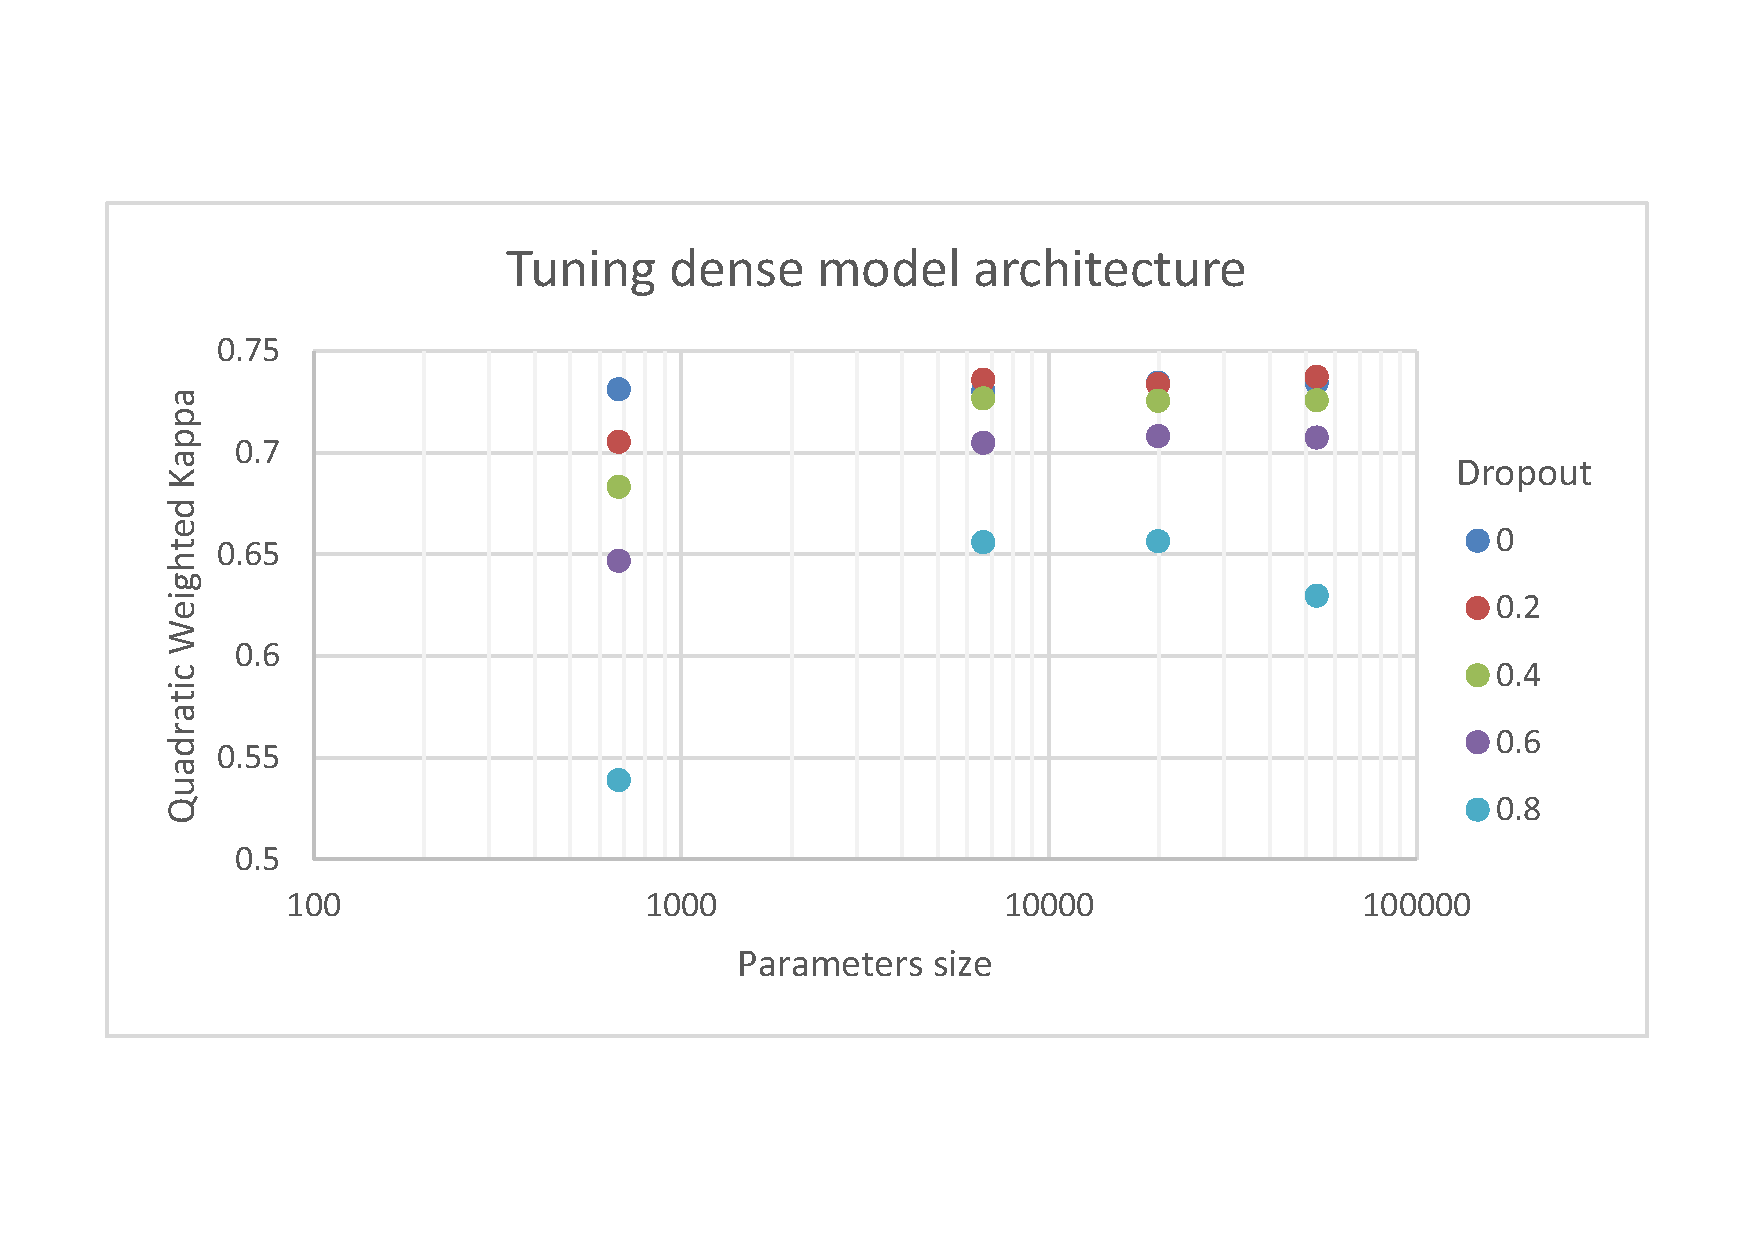
\includegraphics[width=0.85\textwidth]{fig/tune_dense_arch.pdf}
\vspace*{-1.5cm}
\end{center}

\paragraph{LSTM model optimization} We conducted similar experiments for our LSTM model. The best LSTM model was obtained with hidden layer size of $100$ for the recurrent units and $16$ for the fully connected part and droupout value of $0.2$. We then tried deeper model architectures by stacking recurrent units on top of each other. Results show that a depth of $4$ is optimal in our case.

\begin{center}
\vspace*{-1.5cm}
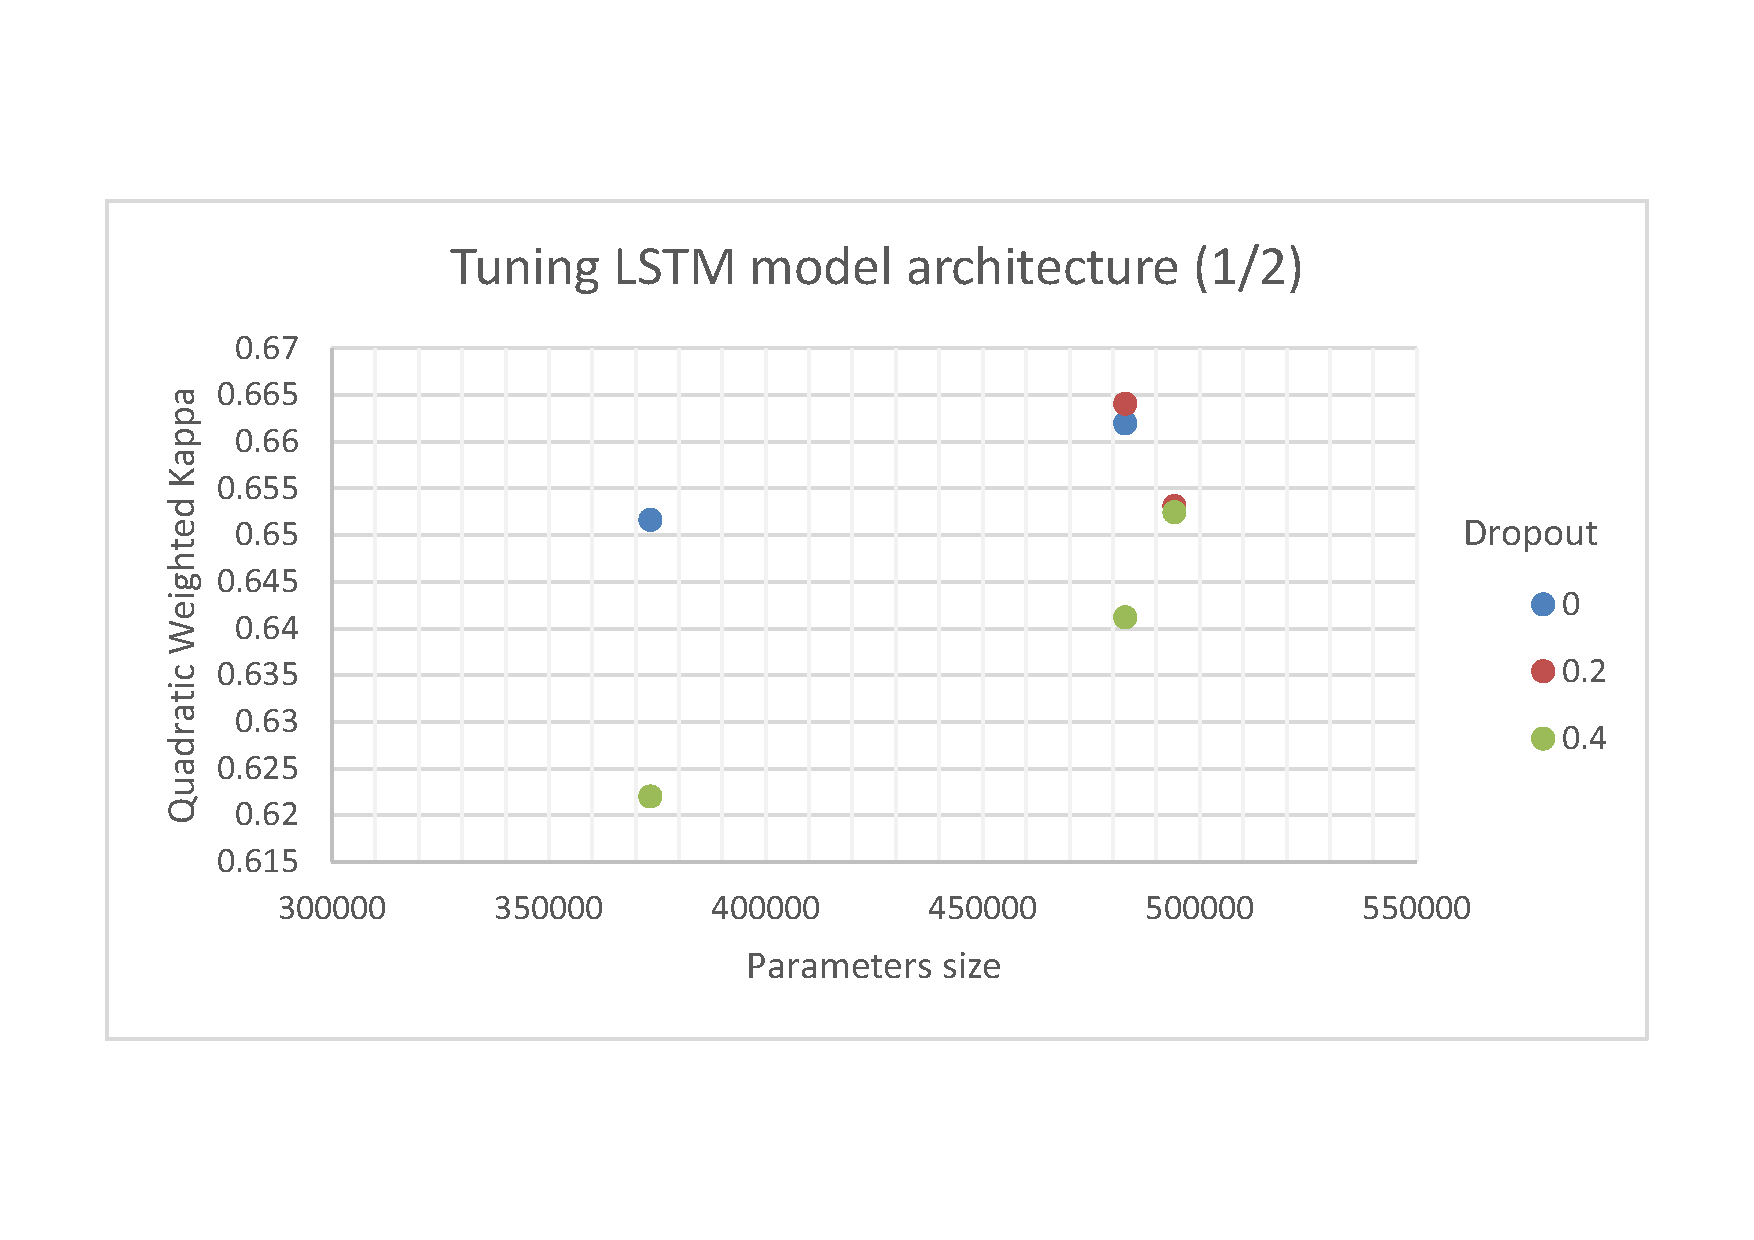
\includegraphics[width=0.85\textwidth]{fig/tune_lstm_arch_1.pdf}
\vspace*{-1.5cm}
\end{center}

\begin{center}
\vspace*{-1.5cm}
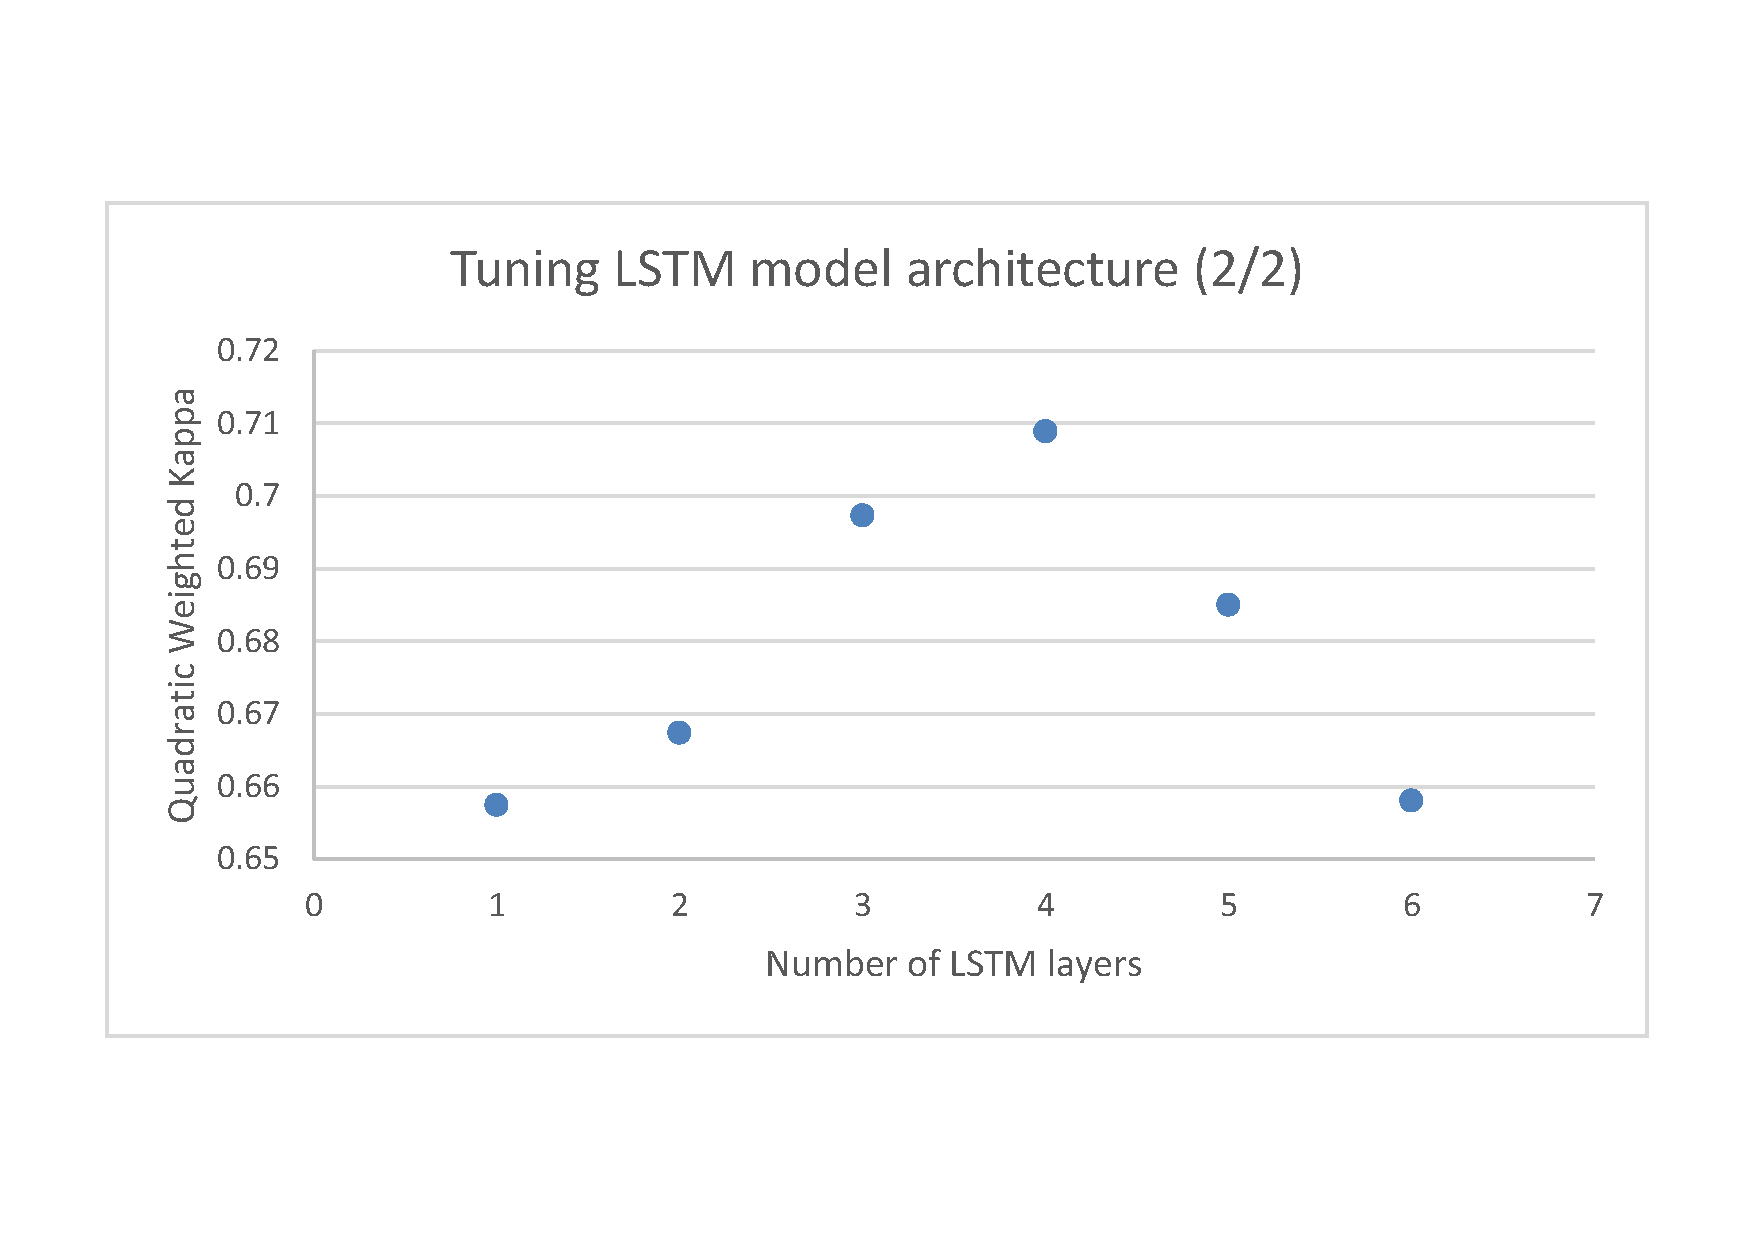
\includegraphics[width=0.85\textwidth]{fig/tune_lstm_arch_2.pdf}
\vspace*{-1.5cm}
\end{center}

\paragraph{CNN model optimization}
We tested only one architecture for the CNN and did not try vary the weights or the number of layers. The main parameter we tuned was dropout. Indeed, a 0 dropout seemed to result in quick overfitting, and increasing dropout helped reduce it. The optimal value for dropout for our model is $0.2$, but even with this, this model is the least performing: on the validation set, the weighted kappa tops at 0.62, whereas dense models can achieve 0.74. More particularly, the CNN is outperformed in all the essay sets by other architectures. The way we interpret this result is that local structure is not predominant in the grading of the essays, and a larger essay-wise view is very beneficial.
\begin{center}
\vspace*{-1.5cm}
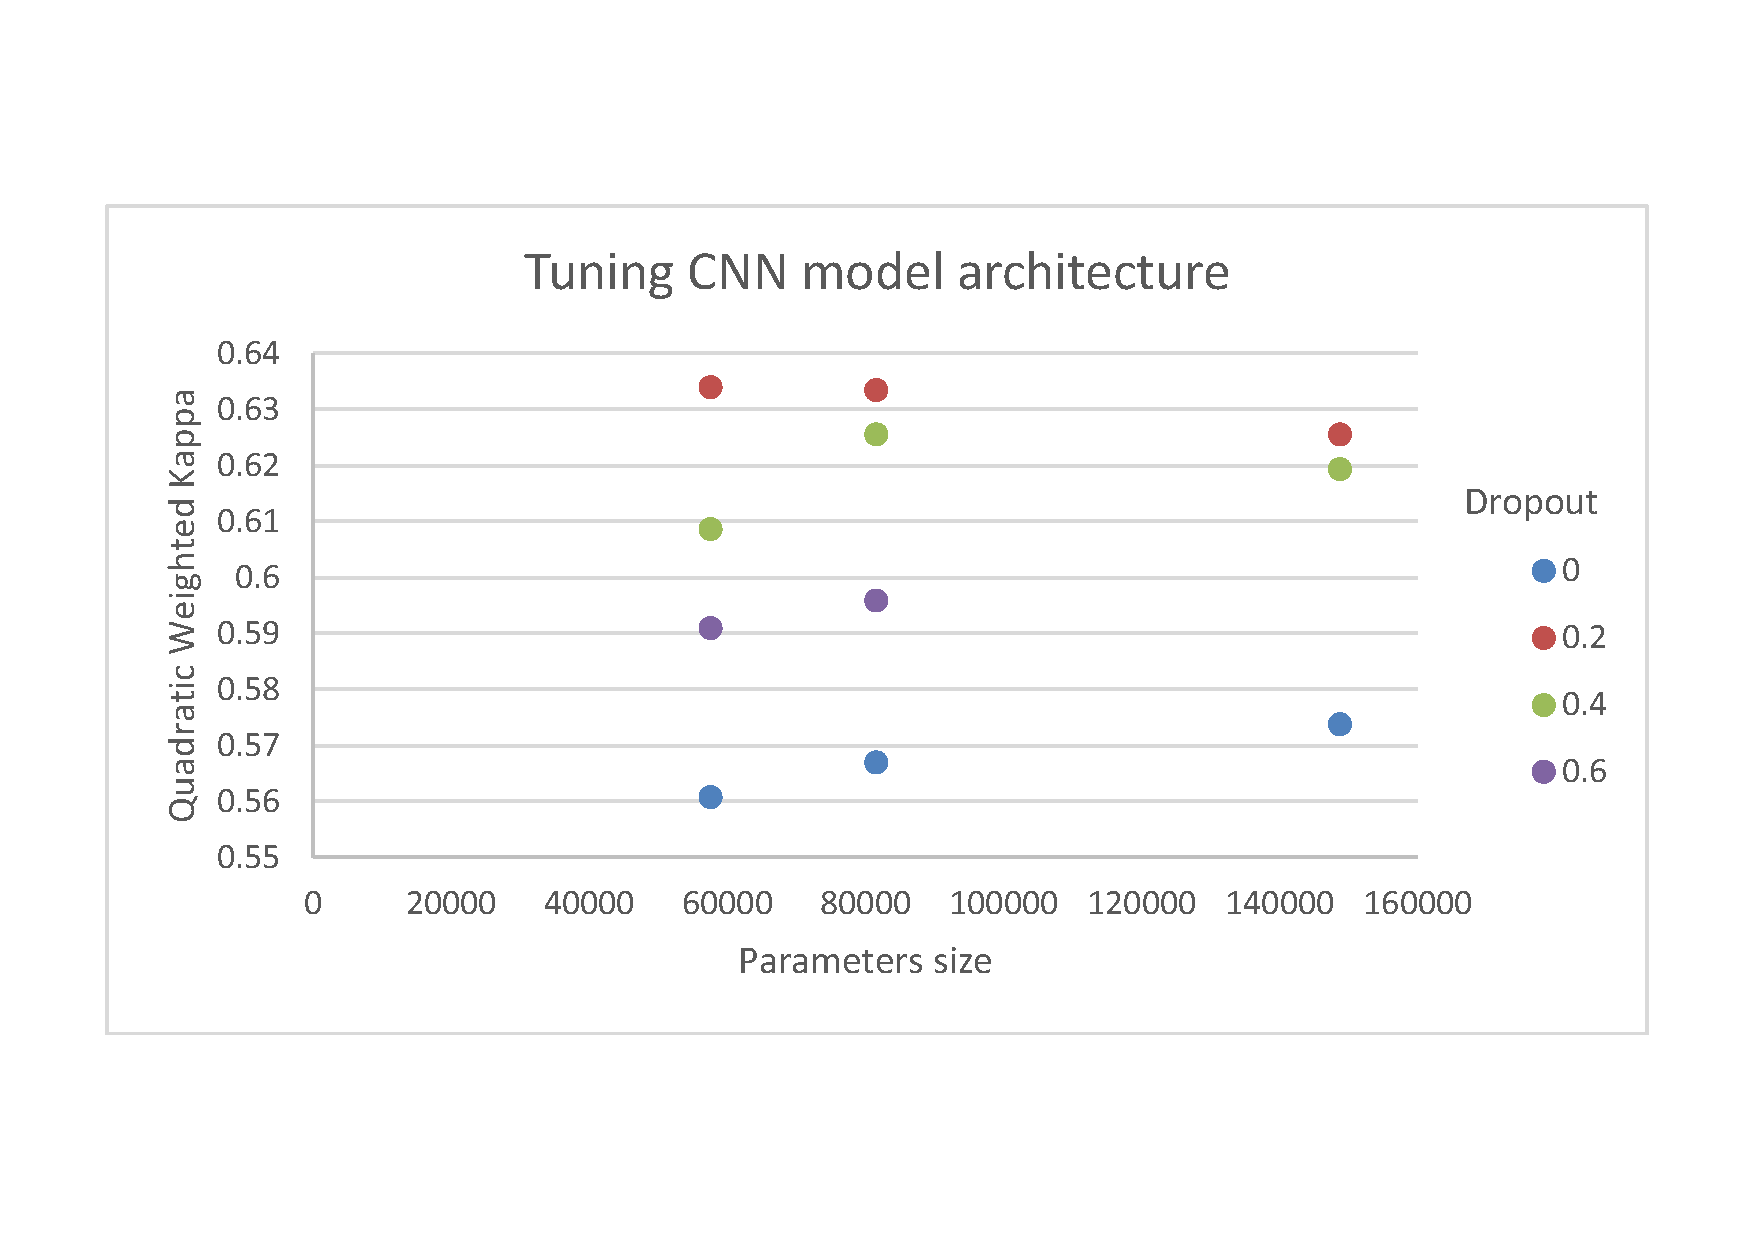
\includegraphics[width=0.85\textwidth]{fig/tune_cnn_arch.pdf}
\vspace*{-1.5cm}
\end{center}


\paragraph{Joint vs individual models} Multitask models are increasingly popular because achieving a good performance level for one task can help tackling other tasks. However, when we compare the results for our joint model compared to the results of individual models we achieve similar performance. Indeed, the quadratic weighted kappa for the joint model is $0.741$ and $0.744$ when compiling results together for individual models. The small difference is due to the joint model not being very good on the $8$\textsuperscript{th} essay set due to size imbalance between sets. Nevertheless, we prefer to keep the joint model as it is much faster to train and less likely to overfit.

\begin{figure}
\centering
% \vspace*{-1.5cm}
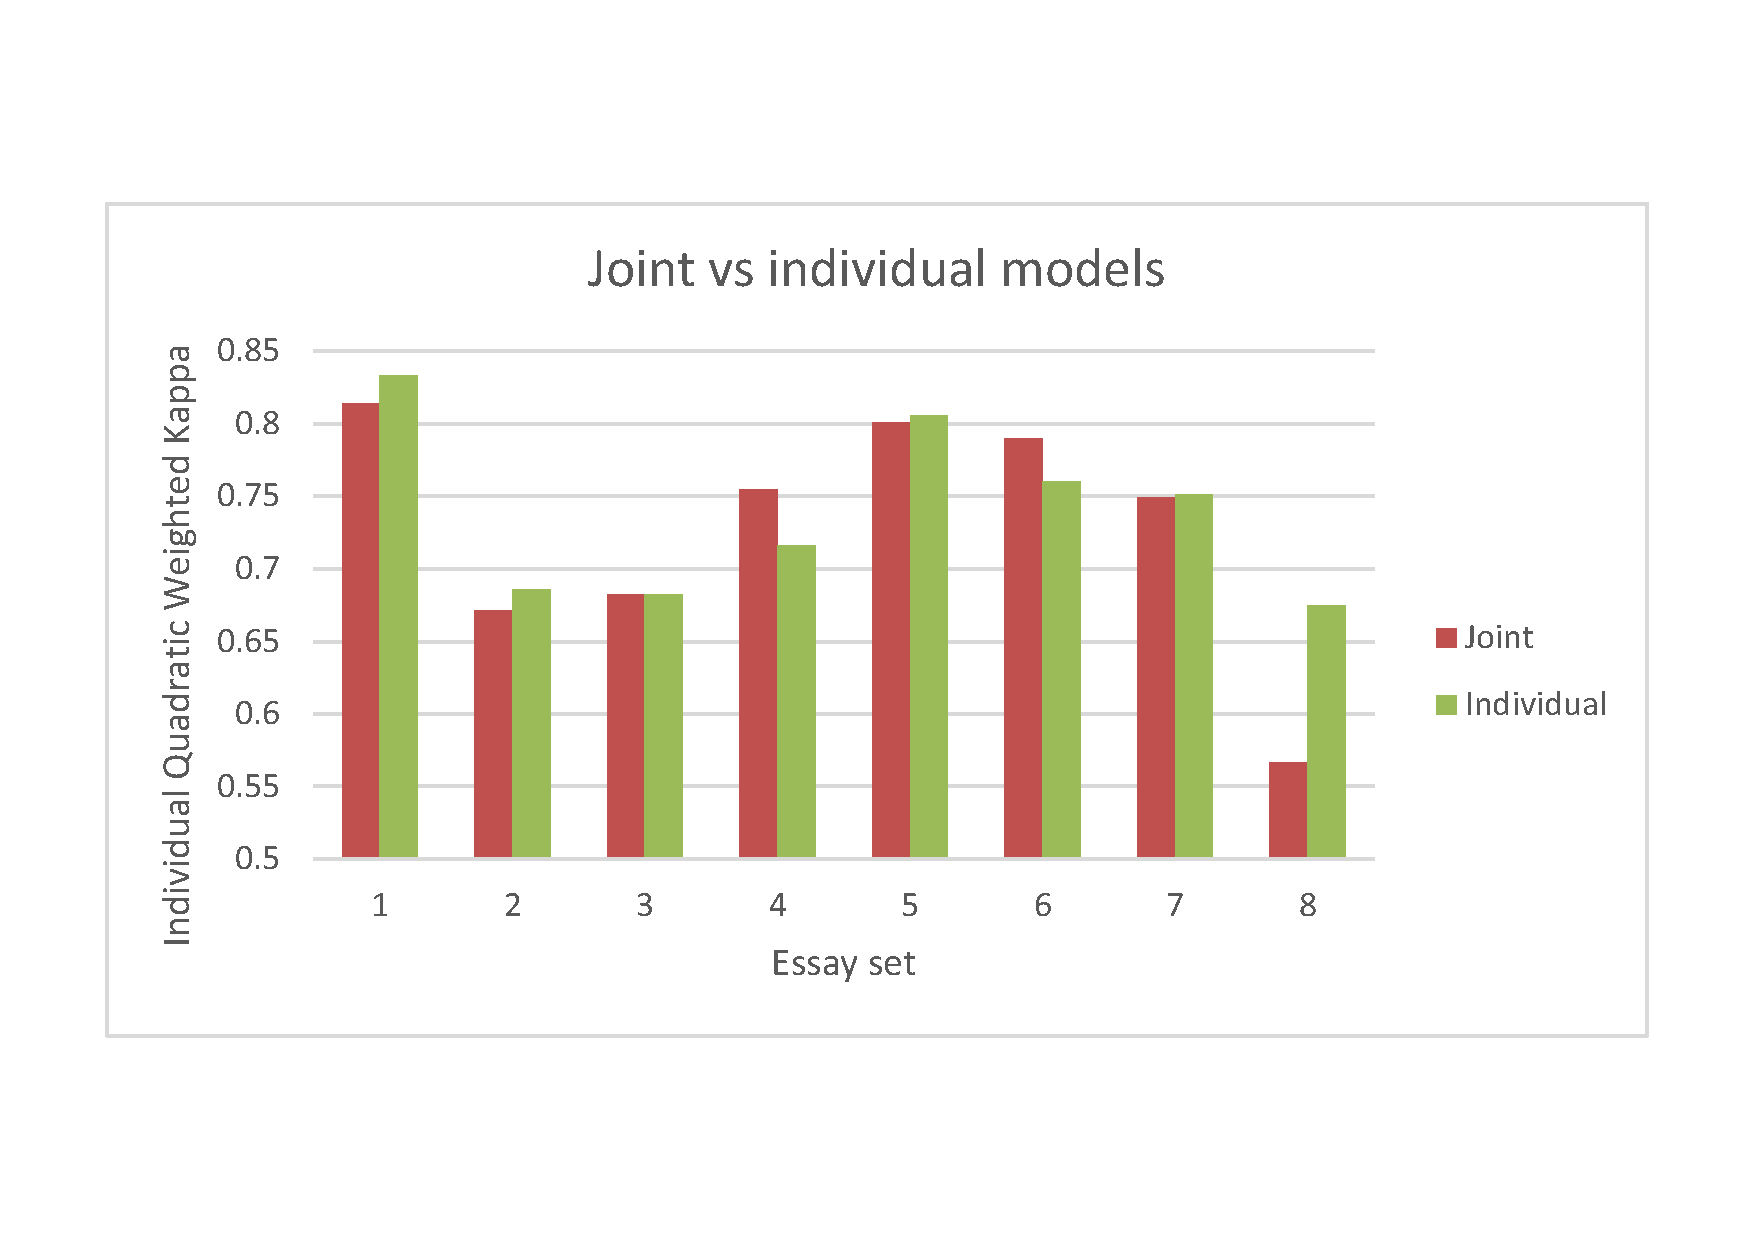
\includegraphics[width=0.85\textwidth]{fig/joint_vs_indiv.pdf}
% \vspace*{-1.5cm}
\caption{Individual performances for each set on the validation and test sets.}
\label{fig:individualperf}
\end{figure}

\paragraph{Word embeddings comparison} We compare all the proposed word embedding strategies. It turns out that the most successful word embedding strategy is the Word2Vec embedding trained on the essay sentences. We think this is due to specific words and contexts being good indicators for the value of an essay. This strategy leverages the whole corpus thus having task specific knowledge for each of the essay tasks.

\begin{center}
\vspace*{-1.5cm}
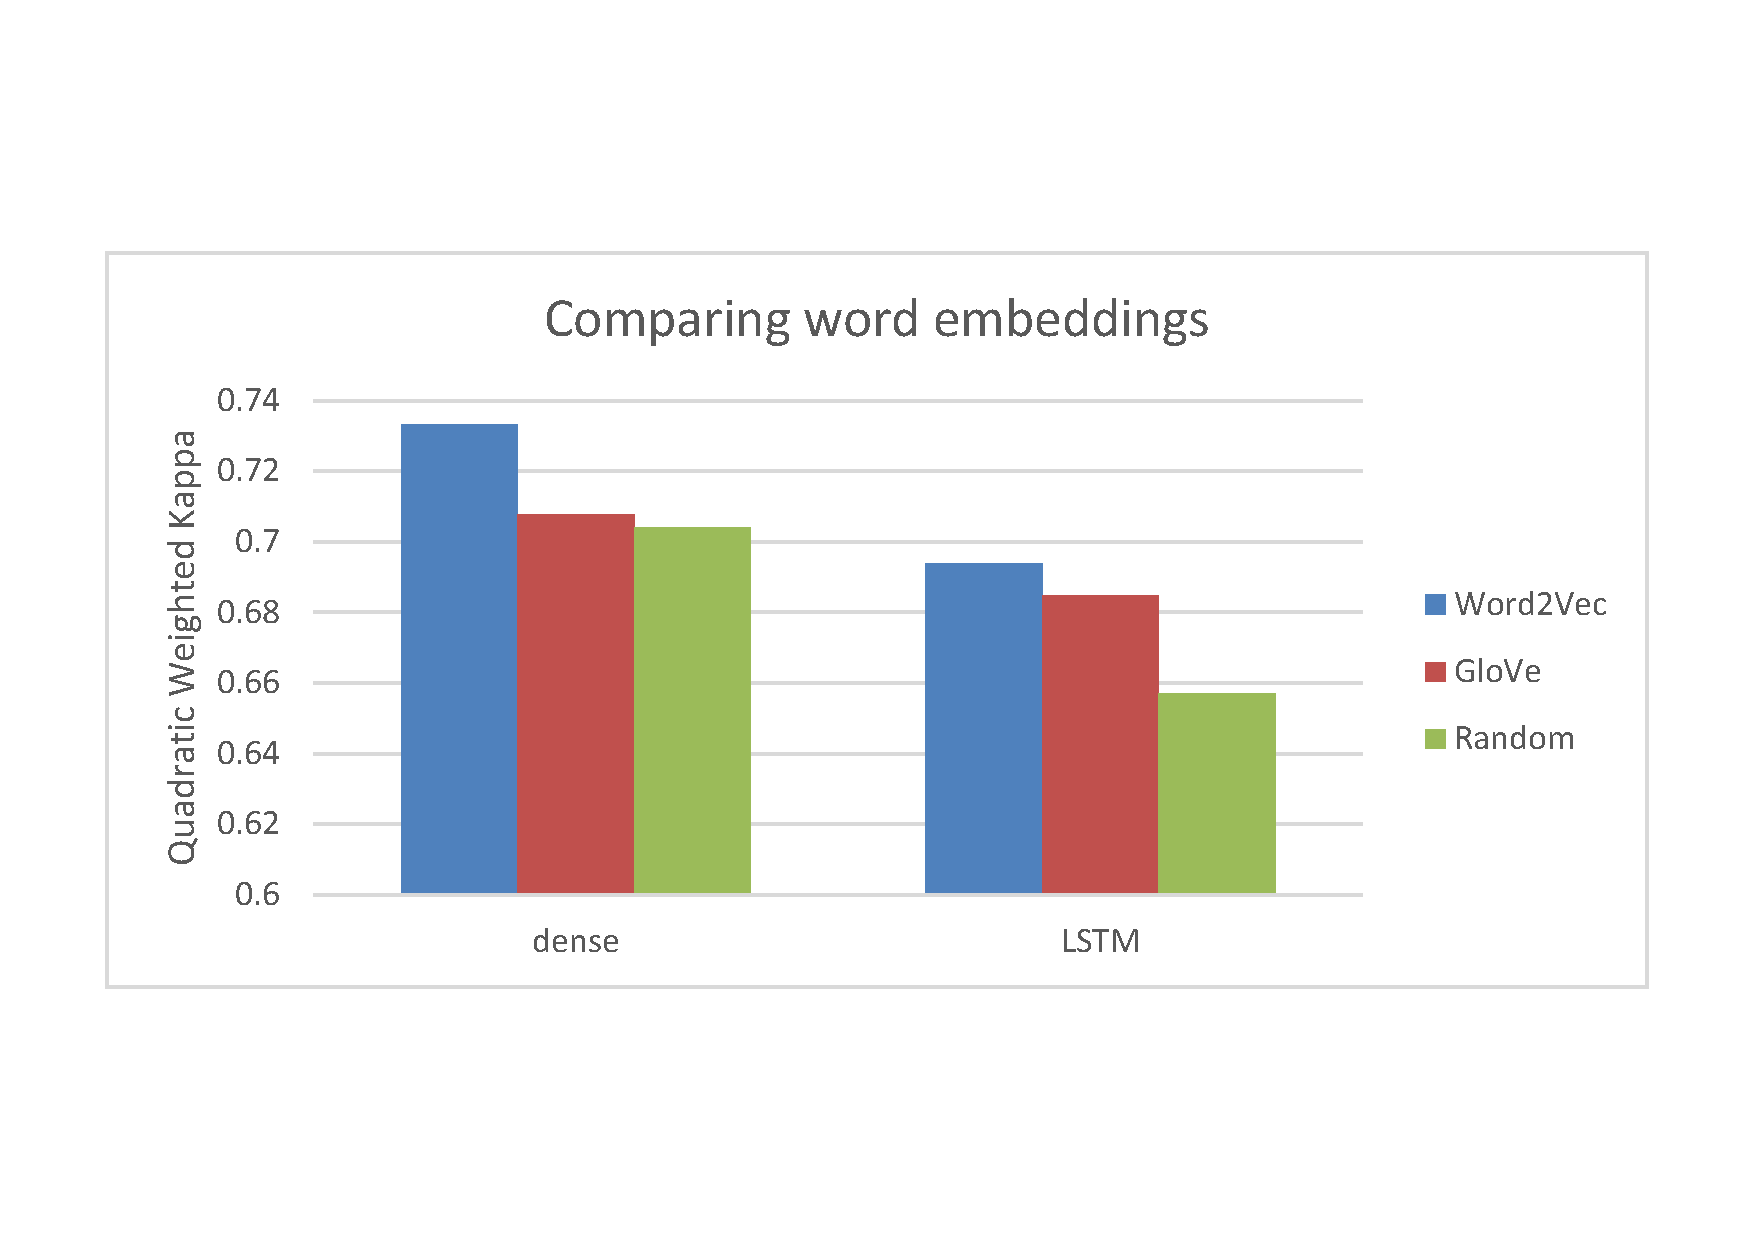
\includegraphics[width=0.85\textwidth]{fig/word_embeddings.pdf}
\vspace*{-1.5cm}
\end{center}

\subsubsection{Best model performance analysis}
The previous section shows that our best performing model has the dense architecture, a word2vec embedding and some dropout. Now, we evaluate the performance of this model on the test data - which has not been used until this point -, compare it with the competition's results, and provide a brief heuristical analysis about the keywords detected by our model.

\paragraph{Test results} We show the performance of the best model on the test set compared to the performance on the validation set. The individual quadratic weighted kappa are equivalent for all sets except the last one. The reason for this is that the score range is the largest for the 8\textsuperscript{th} set and the kappa metric is expecting identical scores to count true positives. So even if the scores are close the kappa can be low. Moreover the 8\textsuperscript{th} set contains less training samples so it is harder to generalize to unseen essays for this set. All in all, the overall performance is quite satisfying and comparable to other works dedicated to this Kaggle competition.

\begin{center}
\vspace*{-1.5cm}
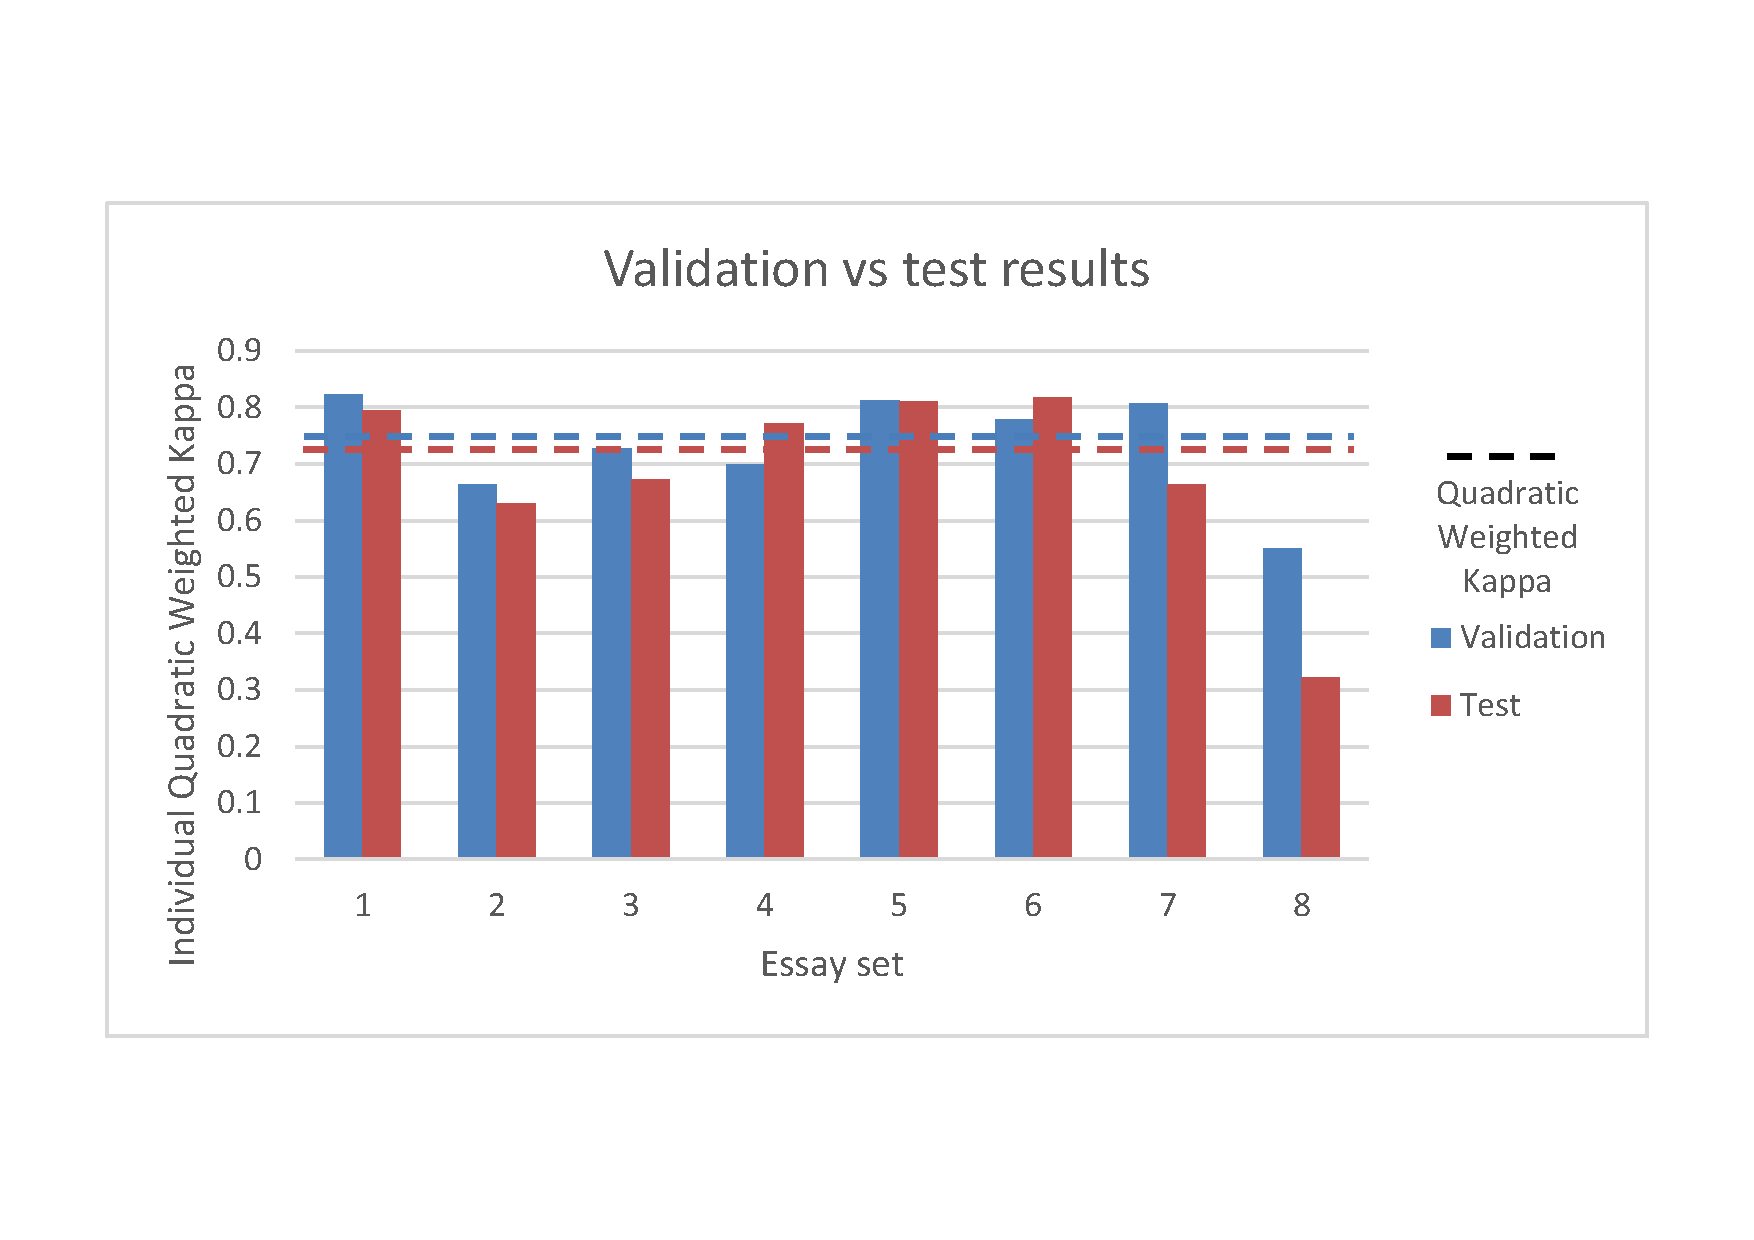
\includegraphics[width=0.85\textwidth]{fig/test.pdf}
\vspace*{-1.5cm}
\end{center}

\paragraph{Words sensitivity analysis} We propose here a simple idea to analyse the sensitivity of our model to particular keywords. We recall from Section~\ref{pos:densearchi} that the dense model starts by averaging all of the embeddings of the essay, and thakes this mean embedding as the input of the dense layers. Hence, it is very easy to feed only one word to the model. Heuristically, this corresponds to automatically grading the essay composed of this sole word. By doing that for all words in the vocabulary, we can map a grade to each word, and analyze this grade as the importance given by the algorithm to this word.
\subparagraph{Caveat - a word on extra features} This simple reasoning is only valid if the only input to the model is the essay's mean embedding. As a matter of fact, our model also requires the extra features described in Section~\ref{pos:extrafeats}. To make the model operate near its training zone and have meaningful results, we do the following : for each set, set each extra feature to its mean value across the set, and feed the embedding of the word as the input. The output of this algorithm is, for each word, a set of grades. However, it is now \emph{wrong} to interpret these grades as "the grade given by the algorithm for essay set number $k$ to the essay consisting of the sole keyword". We will keep that in mind, but neglect it in the analysis.
\subparagraph{Grades of one-word essays} The results of this algorithm are shown in Figure~\ref{fig:onewordessays}. Very interestingly, one can see that it is possible to totally fool the algorithm with essays composed of only one particularly well-chosen word. While being unsurprising, this result shows that the algorithm is not very robust and is very susceptible to adversarial attacks, and hence not suited to be used in real-world applications.\newline
We can further investigate this figure by noting that the shape of the importance profile of Figure~\ref{fig:importance} does not seem to be correlated with performance. Indeed, Sets 1 and 2 have very similar curves, yet the model performs very differently on these two tasks (see Figure~\ref{fig:individualperf}. \newline
Interestingly, it appears that the model is able to identify more more words that matter only for these topics for Sets 1, 2 and 8 : excluding set 7, these are the sets corresponding to argumentative tasks (Table~\ref{setsdescription}). Once again, this is not correlated with performance, as it can be seen on Figure~\ref{fig:individualperf}.

\begin{figure}
	\begin{subfigure}{\textwidth}
		\centering
		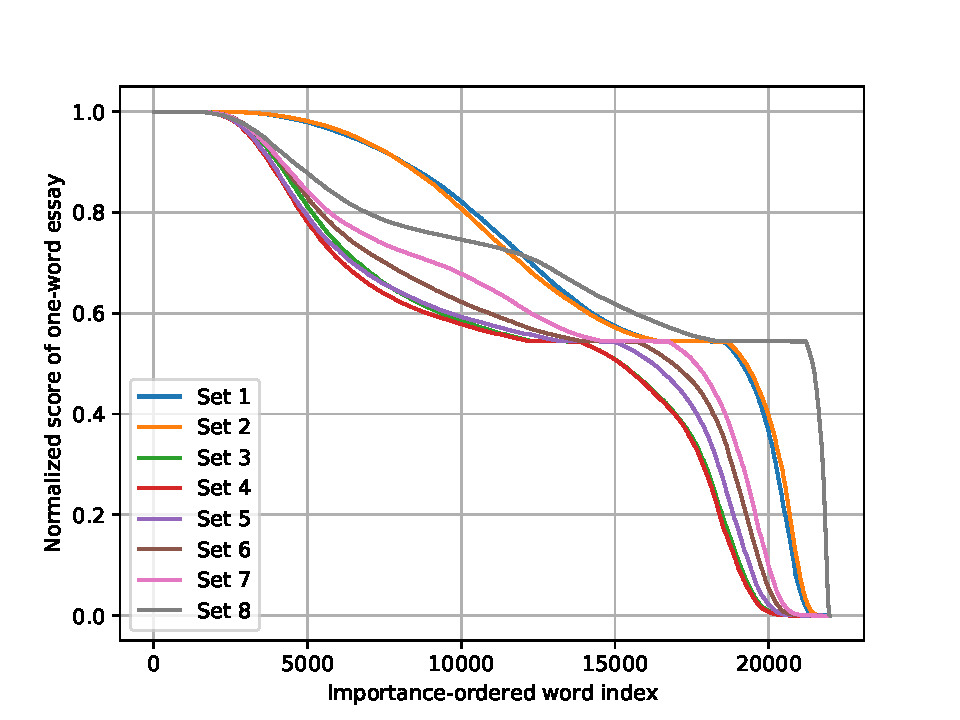
\includegraphics[width=0.8\linewidth]{fig/words_importance.pdf}
		\caption{Sorted words importance.}
		\label{fig:importance}
	\end{subfigure}
	\newline
	\begin{subfigure}{.5\textwidth}
		\centering
		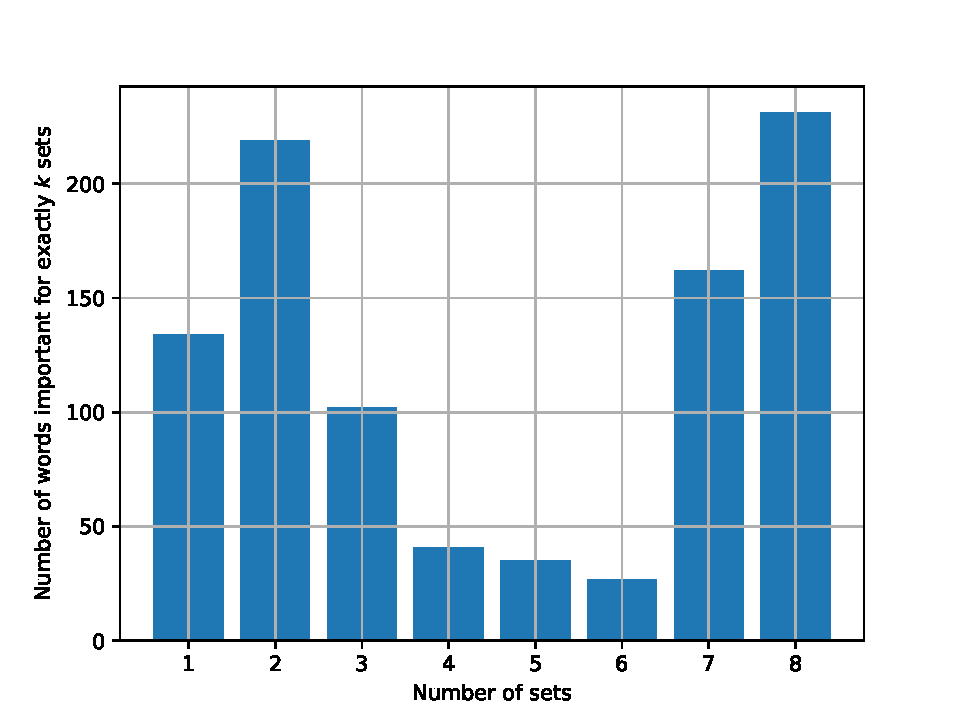
\includegraphics[width=0.8\linewidth]{fig/words_important_in_k_sets.pdf}
		\caption{Words with importance of $1.0$ in exactly $k$ sets.}
		\label{fig:exactlyk}
	\end{subfigure}
	\begin{subfigure}{.5\textwidth}
		\centering
		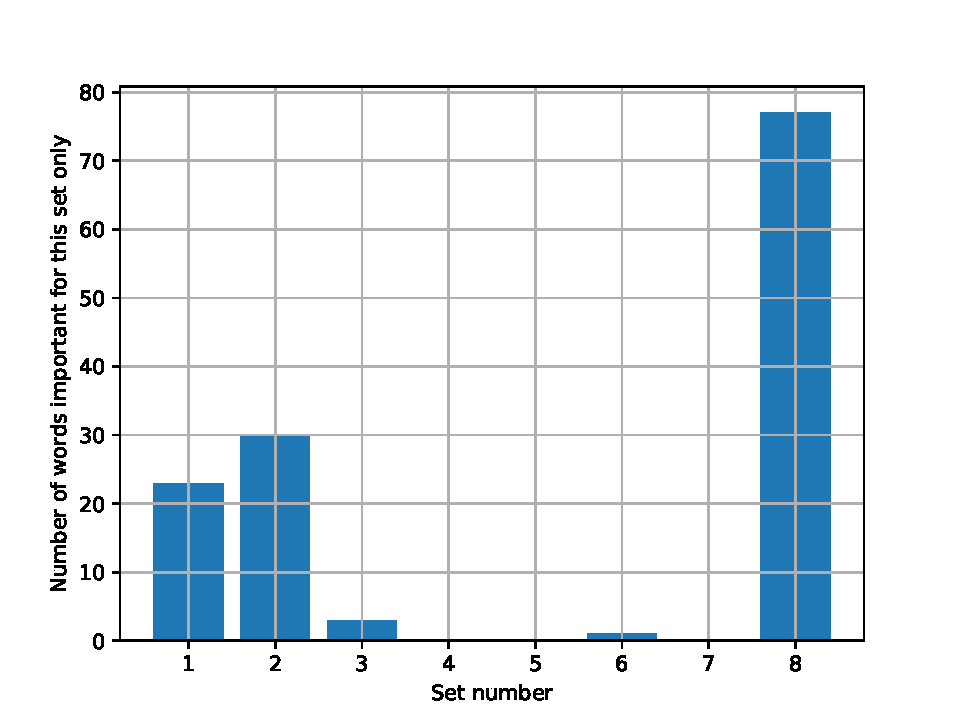
\includegraphics[width=0.8\linewidth]{fig/words_important_only_for_k.pdf}
		\caption{Words with importance of $1.0$ for set $k$ only.}
		\label{fig:onlyk}
	\end{subfigure}
	\caption{Results of the importance algorithm. Figure~\ref{fig:importance} is plotted after sorting the importances independently for each set. Hence, the word corresponding to an index depends on the set. Figures~\ref{fig:exactlyk} and \ref{fig:onlyk} give information on the correlation between the important words across sets.}
	\label{fig:onewordessays}
\end{figure}

\subparagraph{Comparing topics and important words} You will find in Annex~\ref{pos:importantwords} an overview of the important words for sets 1,2 and 8. Surprisingly, most of the words are not specific to the topic upon wich the essay is about, although there are some that match. What's more, some words marked as important have spelling mistakes\footnote{Although this could be accounted for by our spelling error correction algorithm}, such as "teconogly" instead of "technology" for Set 1, "netflicks" instead of "netflix", or even abbreviations or slang talk such as "bf" instead of "boyfriend", or "ganna" that probably stands for "going to". This is probably accounted for by the fact that the dataset is relatively small for deep learning tasks, and more training examples would probably reduce this phenomenon.


\section{Conclusion}
We have started this report by stating how much of a game changer could be a reliable automated scoring system. This project has shown us how difficult designing such a system can be, even with the wonderful toolbox offered by modern natural language processing techniques. By testing several algorithms, we ranked 23rd\footnote{By extrapolating the results obtained on our own test set to the competition's true one, to which we don't have access.} on the competition's leaderboard, yet our algorithm could be easily tricked into giving a high grade to nonsensical essays. It is clear that the basic architecture of the model as well as the small size of the dataset are at fault here, since we cannot reasonably hope for our model to learn grammar. However, gathering more data for such a task is very costly. Indeed, contrary to translation tasks where huge databases can be constituted using existing texts, tests on a particular topic are generally taken only by a handful of students (it is not common for more than a few thousand students to work on the same test), and the resulting essays are generally handwritten and not adapted to being processed by computers. Finally, it requires a lot of human work to rate an essay, much more than to label an image for instance. Hence, even with a better architecture and more computer power, the constitution of the dataset will still be a problem.\par
In spite of all that, this project has helped us shed light on some of the criticisms that were made to automated scoring systems in the past years. It is true that learning-based algorithms primarily focus on structural and formal features that do not necessarily reflect the meaning of the sentence. In our case, this was very obvious, but more sophisticated algorithms are not immuned to this. However, this does not mean that learning algorithms will never be useful for grading. One can imagine a combination of human rating and automated rating to detect rating errors, or use learning-based algorithms for what they are really good at : detecting structures in data, by checking for instance the grammatical correctness of an essay, or other task that largely rely on these surface features that neural networks can detect.

\appendix
\newpage
\section{Important words}
\label{pos:importantwords}
The results presented here can be found in the folder \verb+outputs/000001/processed/+ of the GitHub page of our project.
\subsection{For set 1}
\paragraph{Topic} Write a letter to your local newspaper in which you state your opinion on the effects computers have on people.
\paragraph{Words}
adulterated, appointed, attainable, beards, doesnt, extravagant, 
freer, gunk, haren, jim, loathe, marble, mooned, nerd, 
portals, proceeds, shimmered, teconogly, treadmills, twinkle, unpronounceable, unsocial, venting

\subsection{For set 2}
\paragraph{Topic} Write a persuasive essay to a newspaper reflecting your vies on censorship in libraries.

\paragraph{Words}
anythingelse, athe, carie, ceilings, deflating, durning, eto, frombeing, hardworked, hordes, impressive, moutain, mover, muster, netflicks, overworked, prevails, redon, restated, snooty, solider, sprawled, squires, strats, thistle, tracked, trown, vaccine, watchin, weakly

\subsection{For set 8}
\paragraph{Topic} Tell a true story in which laughter was one element or part.
\paragraph{Words}
appicatrone, aprons, arjuna, ash, bad, bf, building, bup, calorie, cashews, cheeses, comit, contradiction, crazy, dace, detected, exaggerate, extravaganza, figer, funny, ganna, get, girls, go, guy, guys, heartfilling, history, hogweed, hopper,  interviewing, italy, jeopardize, kids, knew, know, let, looked, looking, mauerie, men, might, mom, monstrous, never, older, omg, oppernutity, patient, pediatrician, peeling, pick, pingpong, programe, really, rebuilt, room, satisfies, shaked, shead, shrouded, slur, sometimes, stables, started, store, stray, stuff, suspenseful, tarts, turned, unicycles, unlocks, want, watched, waver, wo


\bibliography{ref} 
\bibliographystyle{ieeetr}
\addcontentsline{toc}{section}{References}

\end{document}